104. а) Катет $QR$ лежит напротив угла в $30^\circ,$ значит $PQ=2QR=13.$ Для точной оценки $QS=PR$ придётся немного забежать вперёд и применить теорему Пифагора: $PR^2+6,5^2=13^2,\ PR^2=126,75.$ Это значит, что длина $QS$ лежит между 11 и 12.\\
б)\begin{figure}[ht!]
\center{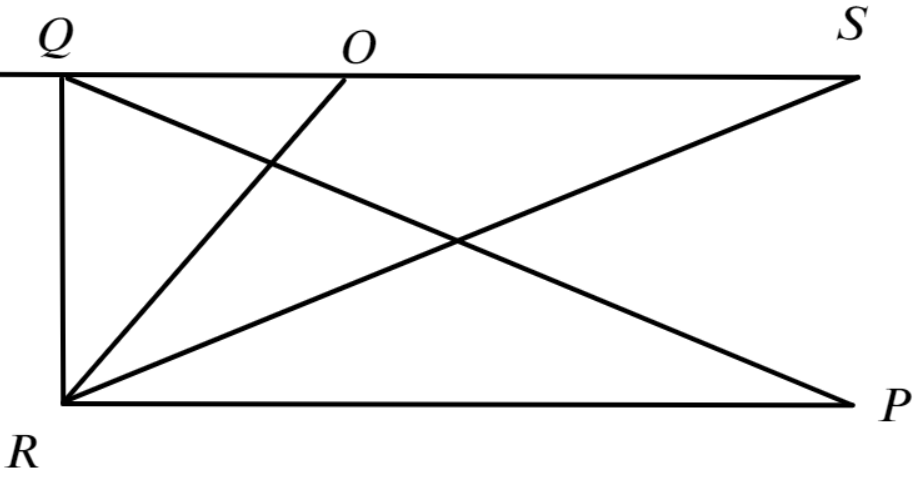
\includegraphics[scale=0.35]{g104.png}}
\end{figure}\\
Треугольники $RQS$ и $RQP$ равны по двум катетам ($QR$ общий, $QS=RP),$ значит $\angle QRS=\angle RQP=60^\circ.$ Тогда $\angle ORS=60^\circ:2=30^\circ,\ \angle QOR=90^\circ-30^\circ=60^\circ,\ \angle ROS=180^\circ-60^\circ=120^\circ,\ \angle OSR=180^\circ-120^\circ-30^\circ=30^\circ.$ Точка $S$ также может лежать с другой стороны от точки $Q,$ что ничего не меняет, так как получившийся треугольник будет симметричен исходному относительно $QR.$\\
